\documentclass[12pt,a4paper]{article}%字号、纸张大小
% =============== 导言区 ===============
\usepackage[UTF8]{ctex}             % 中文支持
% ===== 数学相关 =====
\usepackage{amsmath}                 % 数学公式环境（align、equation等）
\usepackage{amssymb}                 % 额外数学符号（如\mathbb、R等）
\usepackage{amsfonts}                % 数学字体（如\mathrm、\mathcal等）
\usepackage{mathtools}               % amsmath增强（箭头公式、矩阵环境等）
\usepackage{newtxtext}               % 英文正文字体（Times风格）
\usepackage{newtxmath}               % 英文数学字体（Times风格）

% ===== 页面与排版 =====
\usepackage{geometry}                % 页面尺寸和边距设置
\usepackage{setspace}                 % 行距控制

% ===== 表格与图片 =====
\usepackage{graphicx}                % 图片插入
\usepackage{xcolor}                   % 颜色支持（如 \textcolor{blue}{...}）
\usepackage{array}                   % 表格列格式控制
\usepackage{longtable}               % 跨页长表格
\usepackage{booktabs}                 % 专业三线表（\toprule、\midrule、\bottomrule）
\usepackage{multirow}                % 表格单元格跨行合并
\usepackage{wrapfig}                 % 文字环绕图片
\usepackage{textcomp}                % 特殊符号（如 \textcopyright、\textohm 等）

\usepackage{xparse}                % 带可选参数的自定义环境
\usepackage{environ}               % 环境体捕获（用于 answer 环境）
\usepackage{fancyhdr}              % 页眉页脚（习题集模板使用）
\usepackage{newunicodechar}        % 兼容少量数学题中常见的 Unicode 符号
\usepackage[colorlinks=false,pdfborder={0 0 0}]{hyperref} % 目录与跳转

\graphicspath{{./Images/}{Images/}{../Images/}} % 习题图片搜索路径

\newunicodechar{ⅰ}{\ensuremath{\mathrm{i}}}
\newunicodechar{ⅱ}{\ensuremath{\mathrm{ii}}}
\newunicodechar{ⅲ}{\ensuremath{\mathrm{iii}}}
\newunicodechar{ⅳ}{\ensuremath{\mathrm{iv}}}

% =============== 自定义命令 ===============
% 说明：
% 1. 命令用法中的 [...] 表示可选参数，可以省略；省略时使用默认值。
% 2. 命令用法中的 * 表示星号版本，例如 \QuestionSetSection*{...}，星号不写时使用自动编号版本。
% 3. 文件名、图片名等参数一般写在 {...} 中；图片标题等可选内容写在 [...] 中。

% ===== 题目版式命令 =====
% 选择题选项命令，可选参数控制排版方式；可选参数省略时默认为 [1]。
% 用法：\choices{A}{B}{C}{D} 等价于 \choices[1]{A}{B}{C}{D}，4列横排
% 用法：\choices[2]{A}{B}{C}{D}  2列2行
% 用法：\choices[4]{A}{B}{C}{D}  1列4行（每个选项一行）
\newcommand{\choices}[5][1]{%
  \par
  \ifcase#1\relax
  \or % 1: 4列横排
    \begin{tabular*}{0.8\linewidth}[t]{@{\extracolsep{\fill}}cccc}
      \hspace{2em}A．#2 & B．#3 & C．#4 & D．#5
    \end{tabular*}%
  \or % 2: 2列2行
    \begin{tabular}{p{0.45\linewidth}p{0.45\linewidth}}
      \hspace{2em}A．#2 & B．#3 \\
      \hspace{2em}C．#4 & D．#5
    \end{tabular}%
  \or % 3: 未使用
  \or % 4: 1列4行
    \begin{tabular}{l}
      \hspace{2em}A．#2 \\
      \hspace{2em}B．#3 \\
      \hspace{2em}C．#4 \\
      \hspace{2em}D．#5
    \end{tabular}%
  \fi
}

% 选择题选项括号命令
% 用法：\choiceBox 表示选项括号 (~~~~~~)，使用 \mbox 防止括号被换行拆开
\newcommand{\choiceBox}{\mbox{(~~~~~~)}}

% 下划线填空命令
% 用法：\blank{3cm} 表示长度为 3cm 的下划线，使用 \mbox 防止下划线被换行拆开
\newcommand{\blank}[1]{\underline{\mbox{\hspace{#1}}}}

% ===== 题内图片命令 =====
% 图片均为非浮动排版，适合放在 question 环境中的任意位置
\makeatletter
\newcommand{\MC@questionImageCaption}[1]{%
  \if\relax\detokenize{#1}\relax\else
    \par\smallskip
    {\small #1}%
  \fi
}

% 居中图片
% 用法：\questionImage{image1.png} 等价于 \questionImage[0.45\linewidth]{image1.png}
% 用法：\questionImage[0.6\linewidth]{image1.png} 指定图片宽度
% 用法：\questionImage[0.45\linewidth]{image1.png}[图1] 最后的 [图1] 为可选图片标题
\NewDocumentCommand{\questionImage}{O{0.45\linewidth} m o}{%
  \par\smallskip
  \begin{center}
    \includegraphics[width=#1]{#2}%
    \IfNoValueF{#3}{\MC@questionImageCaption{#3}}%
  \end{center}
  \smallskip
}

% 右图左文局部图文块
% 用法：\begin{questionImageRight}{image1.png}左侧文字\end{questionImageRight}
%      等价于 \begin{questionImageRight}[0.32\linewidth]{image1.png}左侧文字\end{questionImageRight}
% 用法：\begin{questionImageRight}[0.32\linewidth]{image1.png}[图1]左侧文字\end{questionImageRight}
%      [0.32\linewidth] 为右侧图片宽度，[图1] 为可选图片标题
\NewDocumentEnvironment{questionImageRight}{O{0.32\linewidth} m o +b}{%
  \par\smallskip
  \noindent
  \begin{minipage}[t]{\dimexpr\linewidth-#1-1em\relax}
    \vspace{0pt}\raggedright
    #4
  \end{minipage}%
  \hspace{1em}%
  \begin{minipage}[t]{#1}
    \vspace{0pt}\centering
    \includegraphics[width=\linewidth]{#2}%
    \IfNoValueF{#3}{\MC@questionImageCaption{#3}}%
  \end{minipage}%
  \par\smallskip
}{}

% 左图右文局部图文块
% 用法：\begin{questionImageLeft}{image1.png}右侧文字\end{questionImageLeft}
%      等价于 \begin{questionImageLeft}[0.32\linewidth]{image1.png}右侧文字\end{questionImageLeft}
% 用法：\begin{questionImageLeft}[0.32\linewidth]{image1.png}[图1]右侧文字\end{questionImageLeft}
%      [0.32\linewidth] 为左侧图片宽度，[图1] 为可选图片标题
\NewDocumentEnvironment{questionImageLeft}{O{0.32\linewidth} m o +b}{%
  \par\smallskip
  \noindent
  \begin{minipage}[t]{#1}
    \vspace{0pt}\centering
    \includegraphics[width=\linewidth]{#2}%
    \IfNoValueF{#3}{\MC@questionImageCaption{#3}}%
  \end{minipage}%
  \hspace{1em}%
  \begin{minipage}[t]{\dimexpr\linewidth-#1-1em\relax}
    \vspace{0pt}\raggedright
    #4
  \end{minipage}%
  \par\smallskip
}{}

% 双图并排
% 用法：\questionImagePair{imageA.png}{imageB.png}
%      等价于 \questionImagePair[0.45\linewidth]{imageA.png}{imageB.png}
% 用法：\questionImagePair[0.45\linewidth]{imageA.png}[图1]{imageB.png}[图2]
%      [0.45\linewidth] 为每张图片宽度，[图1]、[图2] 为可选图片标题
\NewDocumentCommand{\questionImagePair}{O{0.45\linewidth} m o m o}{%
  \par\smallskip
  \noindent
  \begin{minipage}[t]{#1}
    \vspace{0pt}\centering
    \includegraphics[width=\linewidth]{#2}%
    \IfNoValueF{#3}{\MC@questionImageCaption{#3}}%
  \end{minipage}%
  \hfill
  \begin{minipage}[t]{#1}
    \vspace{0pt}\centering
    \includegraphics[width=\linewidth]{#4}%
    \IfNoValueF{#5}{\MC@questionImageCaption{#5}}%
  \end{minipage}%
  \par\smallskip
}
\makeatother

% ===== 答案显示模式 =====
\newif\ifshowans
\newif\ifshowanalysis
\newif\ifchapteranswers
\newif\ifbookanswers
\showansfalse
\showanalysistrue
\chapteranswerstrue
\bookanswersfalse

% 开启题后显示答案功能（主要用于试卷入口 ExamPaper.tex）
% 用法：\showAnswers        显示答案和分析
% 用法：\showAnswersOnly    只显示答案，不显示分析
% 用法：\hideAnswers        隐藏题后答案
\newcommand{\showAnswers}{\global\showanstrue\global\showanalysistrue}
\newcommand{\showAnswersOnly}{\global\showanstrue\global\showanalysisfalse}
\newcommand{\hideAnswers}{\global\showansfalse}

% 习题集常用答案方案（主要用于 QuestionSet.tex，每次只选一种）
% 用法：\answersNone              不显示任何答案
% 用法：\answersByChapter         题后不显示答案，每章末尾显示答案速校
% 用法：\answersAtEnd             题后和章末不显示答案，全书末尾显示答案速校
% 用法：\answersInline            每题后显示答案和分析
% 用法：\answersInlineBrief       每题后只显示答案
% 用法：\answersInlineAndChapter  每题后显示答案和分析，并在章末显示答案速校
% 用法：\studentBook              等价于 \answersByChapter
% 用法：\teacherBook              等价于 \answersInline
\newcommand{\answersNone}{%
  \global\showansfalse
  \global\chapteranswersfalse
  \global\bookanswersfalse
}
\newcommand{\answersByChapter}{%
  \global\showansfalse
  \global\chapteranswerstrue
  \global\bookanswersfalse
}
\newcommand{\answersAtEnd}{%
  \global\showansfalse
  \global\chapteranswersfalse
  \global\bookanswerstrue
}
\newcommand{\answersInline}{%
  \global\showanstrue
  \global\showanalysistrue
  \global\chapteranswersfalse
  \global\bookanswersfalse
}
\newcommand{\answersInlineBrief}{%
  \global\showanstrue
  \global\showanalysisfalse
  \global\chapteranswersfalse
  \global\bookanswersfalse
}
\newcommand{\answersInlineAndChapter}{%
  \global\showanstrue
  \global\showanalysistrue
  \global\chapteranswerstrue
  \global\bookanswersfalse
}
\newcommand{\studentBook}{\answersByChapter}
\newcommand{\teacherBook}{\answersInline}

% 解答题空白区域命令
% 用法：\solutionSpace{5cm} 留出 5cm 答题空间；显示题后答案时自动不留大块空白
\newcommand{\solutionSpace}[1]{%
  \ifshowans
    \par\smallskip
  \else
    \vspace{#1}\par
  \fi
}

% 自动标号计数器
\newcounter{qno}
\newcounter{questionSetChapterNumber}
\newcounter{questionSetSectionNumber}

% 题目环境（替代 \Q{} 的推荐用法）
% 用法：\begin{question}题干内容\end{question} 自动递增题号
% 用法：\begin{question}[题源]题干内容\end{question} 可选参数 [题源] 会显示在题号后
% 使用 begin/end 环境，解决长题目花括号匹配困难的问题
\NewDocumentEnvironment{question}{O{}}{%
  \stepcounter{qno}%
  \raggedright
  \theqno．%
  \if\relax\detokenize{#1}\relax\else（#1）\fi
  \ignorespaces
}{\par}

% 重置题号命令
% 用法：\resetQuestionNumber 将题号重置为 0；通常由 \QuestionSetSection 自动调用
\newcommand{\resetQuestionNumber}{%
  \setcounter{qno}{0}%
}

% ===== 标题与答案命令 =====
\makeatletter
\newcommand{\chapteranswerlist}{}
\newcommand{\bookanswerlist}{}
\let\aclist\chapteranswerlist
\newif\ifsectionanswergroups
\sectionanswergroupsfalse

% 记录大题分组
\newcommand{\ACGroup}[1]{%
  \g@addto@macro\chapteranswerlist{%
    \par\smallskip
    \noindent\textbf{#1}\par
    \noindent
  }%
  \g@addto@macro\bookanswerlist{%
    \par\smallskip
    \noindent\textbf{#1}\par
    \noindent
  }%
}

% 记录单题答案
\newcommand{\ACItem}[2]{%
  \g@addto@macro\chapteranswerlist{%
    \textbf{#1.}~#2\qquad
  }%
  \g@addto@macro\bookanswerlist{%
    \textbf{#1.}~#2\qquad
  }%
}

% 大题标题命令
% 用法：\questionGroup{标题内容} 输出加粗大题标题，并把标题写入答案速校分组
\newcommand{\questionGroup}[1]{%
  \ifsectionanswergroups\else
    \ACGroup{#1}%
  \fi
  \noindent\textbf{#1}\par
}

% 答案环境（替代 \A{答案}{分析}）
% 用法：\begin{answer}{答案}分析内容\end{answer}
% 用法：\begin{answer}{答案}\end{answer} 分析为空时不显示【分析】标签
% 第一个花括号参数会进入答案速校；环境正文是详细分析
\NewEnviron{answer}[1]{%
  \ifshowans
    \par\smallskip
    {\color{red}\textbf{【答案】}}{\boldmath\textbf{#1}}\par
    \ifshowanalysis
      \if\relax\detokenize\expandafter{\BODY}\relax\else
        {\color{red}\textbf{【分析】}}~\BODY\par
      \fi
    \fi
    \vspace{6ex}
  \fi
  \begingroup
    \edef\x{\endgroup
      \noexpand\ACItem{\theqno}{\unexpanded{#1}}%
    }%
  \x
}

% 参考答案页 / 本章答案速校
% 用法：\printAnswerCheck 显示当前已收集的答案速校内容
\newcommand{\printAnswerCheck}{%
    \begingroup
    \small
    \noindent{\large \textbf{答案速校}}\par
    \ifx\chapteranswerlist\@empty
      \noindent（本部分暂无答案。）\par
    \else
      \noindent\chapteranswerlist\par
    \fi
    \endgroup
    \medskip
}

% 用法：\printBookAnswerCheck 在全书末尾输出全书答案速校；仅 \answersAtEnd 模式下生效
\newcommand{\printBookAnswerCheck}{%
  \ifbookanswers
    \clearpage
    \begin{center}
      {\Large\bfseries 全书答案速校}
    \end{center}
    \begingroup
    \small
    \ifx\bookanswerlist\@empty
      \noindent（本书暂无答案。）\par
    \else
      \noindent\bookanswerlist\par
    \fi
    \endgroup
  \fi
}
\makeatother

% ===== 章节结构命令 =====

% 习题集封面、目录与页眉
% 用法：\UseQuestionSetStyle{高中数学习题集} 设置页眉、页脚和页码样式
\newcommand{\UseQuestionSetStyle}[1]{%
  \setlength{\headheight}{15pt}%
  \pagestyle{fancy}
  \fancyhf{}
  \fancyhead[L]{#1}
  \fancyhead[R]{\nouppercase{\leftmark}}
  \fancyfoot[C]{\thepage}
  \renewcommand{\headrulewidth}{0.4pt}
}

% 用法：\QuestionSetCover{主标题}{副标题}{底部信息} 生成习题集封面
\newcommand{\QuestionSetCover}[3]{%
  \begin{titlepage}
    \centering
    \vspace*{0.16\textheight}
    {\Huge\bfseries #1\par}
    \vspace{1.2cm}
    {\Large #2\par}
    \vfill
    {\large #3\par}
  \end{titlepage}
}

% 用法：\QuestionSetTOC 输出目录并自动分页
\newcommand{\QuestionSetTOC}{%
  \clearpage
  \tableofcontents
  \clearpage
}

% 用法：\includeChapter{01-集合与常用逻辑用语}
%      自动输入 chapters/01-集合与常用逻辑用语.tex，不需要写 chapters/ 和 .tex
\newcommand{\includeChapter}[1]{%
  \input{chapters/#1.tex}%
}

\makeatletter
\newcommand{\MC@appendBookChapter}[1]{%
  \g@addto@macro\bookanswerlist{%
    \par\bigskip
    \noindent{\large\bfseries #1}\par
    \smallskip
  }%
}

% 章标题（新页开始，居中大号）
% 用法：\QuestionSetChapter{函数与基本性质} 自动显示“第1章　函数与基本性质”
% 用法：\QuestionSetChapter*{附录} 显示“附录”，不推进章节编号
% 非星号版本会重置小节编号、写入目录、更新页眉，并开始收集本章答案
\NewDocumentCommand{\QuestionSetChapter}{s m}{%
  \clearpage
  \gdef\chapteranswerlist{}%
  \global\sectionanswergroupsfalse
  \IfBooleanTF{#1}{%
    \def\MC@chapterTitle{#2}%
  }{%
    \stepcounter{questionSetChapterNumber}%
    \setcounter{questionSetSectionNumber}{0}%
    \def\MC@chapterTitle{第\arabic{questionSetChapterNumber}章　#2}%
  }%
  \expandafter\MC@appendBookChapter\expandafter{\MC@chapterTitle}%
  \phantomsection
  \addcontentsline{toc}{section}{\MC@chapterTitle}%
  \markboth{\MC@chapterTitle}{\MC@chapterTitle}%
  \begin{center}
    {\Large\bfseries \MC@chapterTitle}
  \end{center}
}

% 节标题（知识点名称，左对齐加粗）
% 用法：\QuestionSetSection{函数的概念与表示} 自动显示“1.1　函数的概念与表示”
% 用法：\QuestionSetSection*{本章综合训练} 显示“本章综合训练”，不推进小节编号
% 非星号版本会递增小节编号；两种版本都会重置题号、写入目录并开启答案分组
\NewDocumentCommand{\QuestionSetSection}{s m}{%
  \par\medskip
  \resetQuestionNumber
  \global\sectionanswergroupstrue
  \IfBooleanTF{#1}{%
    \def\MC@sectionTitle{#2}%
  }{%
    \stepcounter{questionSetSectionNumber}%
    \def\MC@sectionTitle{\arabic{questionSetChapterNumber}.\arabic{questionSetSectionNumber}　#2}%
  }%
  \expandafter\ACGroup\expandafter{\MC@sectionTitle}%
  \phantomsection
  \addcontentsline{toc}{subsection}{\MC@sectionTitle}%
  \noindent{\large\bfseries \MC@sectionTitle}\par
  \smallskip
}

% 本章答案速校 — 显示累积答案后清空，各章答案互不干扰
% 用法：\printChapterAnswers 输出本章答案速校；仅章末答案模式开启时显示
\newcommand{\printChapterAnswers}{%
  \ifchapteranswers
    \clearpage
    \begin{center}
      {\Large\bfseries 本章答案速校}
    \end{center}
    \printAnswerCheck
  \fi
  \gdef\aclist{}%
  \gdef\chapteranswerlist{}%
}
\makeatother

\geometry{a4paper,margin=2cm,top=2cm,bottom=2cm}%页边距
\graphicspath{{./Images/}}        % 图片默认搜索路径（当前目录下的Images文件夹）
\setstretch{1.5}                     % 1.5倍行距
\setlength{\parindent}{0pt}           % 段首缩进（0pt=不缩进）
\setlength{\parskip}{1ex}            % 段落间距

% =============== 自定义命令说明 ===============
% -------- 题目结构 --------
% \begin{question}...\end{question}  % 题目环境（自动编号）
% \questionGroup{大题标题}                    % 大题标题
% \resetQuestionNumber                            % 重置题号计数器
%
% -------- 选择题/填空题 --------
% \choices{A}{B}{C}{D}        % 四选项横排（默认）
% \choices[2]{A}{B}{C}{D}     % 四选项分两行（AB / CD）
% \choices[4]{A}{B}{C}{D}     % 四选项竖排（每个一行）
% \choiceBox                    % 选项括号 (~~~~~~)
% \blank{3cm}               % 下划线填空
%
% -------- 解答题 --------
% \solutionSpace{5cm}             % 留出答题空间
%
% -------- 答案 --------
% \begin{answer}{答案}
%   分析内容（可空，为空时不显示【分析】标签）
% \end{answer}

% =============== 使用\showAnswers后，编译 ExamPaper.tex 时在每题后显示答案 ===============
%\showAnswers

\begin{document}

\begin{center}
	{\Large \textbf{数学校本作业}}

	命题、 审题：

	班级\blank{3cm}姓名\blank{3cm}学号\blank{3cm}
\end{center}


% ==================== 一、选择题 ====================
\questionGroup{一、选择题：本大题共8小题，每小题5分，共计40分.每小题给出的四个选项中，只有一个选项是正确的.请把正确的选项填涂在答题卡相应的位置上.}

% ----------------------------------------
\begin{question}
$(1+5\text{i})\text{i}$的虚部为\choiceBox
\choices{$-1$}{0}{1}{6}
\end{question}
% --- 【答案】---
\begin{answer}{C}
$(1+5i)i=i-5=-5+i$，故虚部为 $1$。选 C。
\end{answer}

% ----------------------------------------
\begin{question}
设全集$U=\left\{ x\mid x<9 \right\}$，集合$A=\{1,3,5\}$，则$\complement_U A$中元素个数为\choiceBox
\choices{0}{3}{5}{8}
\end{question}
% --- 【答案】---
\begin{answer}{C}
全集 $U=\{1,2,3,4,5,6,7,8\}$，$\complement_UA=\{2,4,6,7,8\}$，共 $5$ 个元素。选 C。
\end{answer}

% ----------------------------------------
\begin{question}
若双曲线$C$的虚轴长为实轴长的$\sqrt{7}$倍，则$C$的离心率为\choiceBox
\choices{$\sqrt{2}$}{2}{$\sqrt{7}$}{$2\sqrt{2}$}
\end{question}
% --- 【答案】---
\begin{answer}{D}
设双曲线方程为 $\dfrac{x^2}{a^2}-\dfrac{y^2}{b^2}=1$（$a>0,b>0$），虚轴长 $2b$，实轴长 $2a$。由 $2b=\sqrt{7}\cdot2a$ 得 $b=\sqrt{7}a$，离心率 $e=\dfrac{c}{a}=\sqrt{1+\dfrac{b^2}{a^2}}=\sqrt{8}=2\sqrt{2}$。选 D。
\end{answer}

% ----------------------------------------
\begin{question}
若点$(a,0)(a>0)$是函数$y=2\tan \left( x-\dfrac{\pi}{3} \right)$的图象的一个对称中心，则$a$的最小值为\choiceBox
\choices{$\dfrac{\pi}{6}$}{$\dfrac{\pi}{3}$}{$\dfrac{\pi}{2}$}{$\dfrac{4\pi}{3}$}
\end{question}
% --- 【答案】---
\begin{answer}{B}
正切函数 $y=\tan(x)$ 的对称中心为 $\left(\dfrac{k\pi}{2},0\right),k\in\mathbf{Z}$。令 $x-\dfrac{\pi}{3}=\dfrac{k\pi}{2}$，得 $x=\dfrac{\pi}{3}+\dfrac{k\pi}{2}$，$a>0$ 时 $k=0$ 得 $a=\dfrac{\pi}{3}$。选 B。
\end{answer}

% ----------------------------------------
\begin{question}
设$f(x)$是定义在$\mathbf{R}$上且周期为2的偶函数，当$2\le x\le 3$时，$f(x)=5-2x$，则$f\left( -\dfrac{3}{4} \right)=$\choiceBox
\choices{$\dfrac{1}{2}$}{$-\dfrac{1}{4}$}{$\dfrac{1}{4}$}{$\dfrac{1}{2}$}
\end{question}
% --- 【答案】---
\begin{answer}{A}
$f$ 为周期 $2$ 的偶函数，$f\left(-\dfrac34\right)=f\left(\dfrac34\right)=f\left(\dfrac{11}{4}\right)=5-2\times\dfrac{11}{4}=-\dfrac12$。选 A。
\end{answer}

% ----------------------------------------
\begin{question}
帆船比赛中，运动员可借助风力计测定风速的大小和方向，测出的结果在航海学中称为视风风速，视风风速对应的向量，是真风风速对应的向量与船行风速对应的向量之和，其中船行风速对应的向量与船速对应的向量大小相等，方向相反.图1给出了部分风力等级、名称与风速大小的对应关系.已知某帆船运动员在某时刻测得的视风风速对应的向量与船速对应的向量如图2（风速的大小和向量的大小相同），单位（m/s），则真风为\choiceBox
\begin{center}
	% 左侧：放置图1的表格，占据55%的行宽，垂直居中对齐
	\begin{minipage}[c]{0.55\textwidth}
		\centering
		\begin{tabular}{|c|c|c|}
			\hline
			等级 & 风速大小m/s & 名称 \\ \hline
			2 & 1.1$\sim$3.3 & 轻风 \\ \hline
			3 & 3.4$\sim$5.4 & 微风 \\ \hline
			4 & 5.5$\sim$7.9 & 和风 \\ \hline
			5 & 8.0$\sim$10.1 & 劲风 \\ \hline
		\end{tabular}
	\end{minipage}
	\hfill % 自动填充中间空白，将两边撑开
	% 右侧：放置图2的图片，占据40%的行宽
	\begin{minipage}[c]{0.4\textwidth}
		\centering
		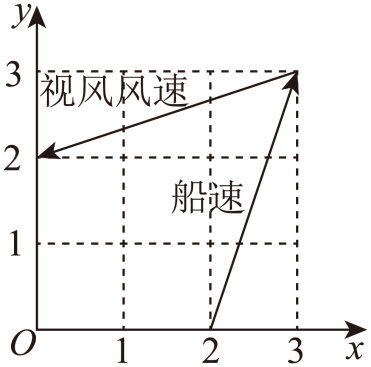
\includegraphics[width=0.6\textwidth]{image1.png}
	\end{minipage}
\end{center}




\choices{轻风}{微风}{和风}{劲风}
\end{question}
% --- 【答案】---
\begin{answer}{A}
视风 $\vec a=(-3,-1)$，船速 $\vec b=(1,3)$，真风 $\vec n=\vec a+\vec b=(-2,2)$，$|\vec n|=\sqrt{8}=2\sqrt2\approx2.828\in[1.6,3.3)$，为轻风。选 A。
\end{answer}

% ----------------------------------------
\begin{question}
若圆$x^2+(y+2)^2=r^2(r>0)$上到直线$y=\sqrt{3}x+2$的距离为1的点有且仅有2个，则$r$的取值范围是\choiceBox



\choices[4]{$(0,1)$}{$(1,3)$}{$(3,+\infty )$}{$(0,+\infty)$}
\end{question}
% --- 【答案】---
\begin{answer}{B}
圆心 $C(0,-2)$，$d_1=1,d_2=3$，当 $1<r<3$ 时圆与 $l_1$ 相交（2点）与 $l_2$ 不相交，共 $2$ 点。选 B。
\end{answer}

% ----------------------------------------
\begin{question}
若实数$x$、$y$、$z$满足$2+\log_2x=3+\log_3y=5+\log_5z$，则$x$、$y$、$z$的大小关系不可能是\choiceBox



\choices[2]{$x>y>z$}{$x>z>y$}{$y>x>z$}{$y>z>x$}
\end{question}
% --- 【答案】---
\begin{answer}{B}
设 $2+\log_2x=3+\log_3y=5+\log_5z=t$，则 $x=2^{t-2},y=3^{t-3},z=5^{t-5}$。$t=8$ 时 $y>z>x$；$t=0$ 时 $x>y>z$；$t=5$ 时 $y>x>z$。故不可能为 B。
\end{answer}


% ==================== 二、选择题 ====================
\questionGroup{二、选择题：本题共3小题，每小题6分，共18分.在每小题给出的选项中，有多项符合题目要求.全部选对的得6分，部分选对的得部分分，有选错的得0分.}

% ----------------------------------------
\begin{question}
在正三棱柱$ABC-A_1B_1C_1$中，D为BC中点，则\choiceBox



\choices[2]{$AD\bot {A}_{1}C$}{$BC\bot\text{平面}A{A}_{1}D$}{$AD//{A}_{1}{B}_{1}$}{$C{C}_{1}//\text{平面}A{A}_{1}D$}
\end{question}
% --- 【答案】---
\begin{answer}{BD}
A：$AD\perp A_1C$ 且 $AD\perp AA_1\Rightarrow AD\perp$ 平面 $AA_1C\Rightarrow AD\perp AC$，矛盾，A 错；B：$AD\perp BC,AA_1\perp BC\Rightarrow BC\perp$ 平面 $AA_1D$，B 正确；C：$AD\parallel A_1B_1$ 与 $AD\parallel A_1D_1$ 矛盾，C 错；D：$CC_1\parallel AA_1$ 且 $CC_1$ 不在平面 $AA_1D$，故 $CC_1\parallel$ 平面 $AA_1D$，D 正确。选 BD。
\end{answer}

% ----------------------------------------
\begin{question}
设抛物线$C:y^2=6x$的焦点为$F$，过$F$的直线交$C$于$A$、$B$，过$F$且垂直于$AB$的直线交$l:x=-\dfrac{3}{2}$于$E$，过点$A$作准线$l$的垂线，垂足为$D$，则\choiceBox



\choices[2]{$|AD|=|AF|$}{$|AE|=|AB|$}{$|AB|\ge 6$}{$|AE|\cdot|BE|\ge 18$}
\end{question}
% --- 【答案】---
\begin{answer}{AC}
A：抛物线定义 $|AD|=|AF|$，A 正确；B：取通径 $A(\dfrac32,3),B(\dfrac32,-3)$，$AB=6\neq AE$，B 错；C：焦点弦 $|AB|\ge2p=6$，C 正确；D：$|AE|\cdot|BE|\ge18$，当 $m=0$ 时取等，D 正确。选 ACD。
\end{answer}

% ----------------------------------------
\begin{question}
已知$\triangle ABC$的面积为$\dfrac{1}{4}$，若$\cos 2A+\cos 2B+2\sin C=2,\cos A\cos B\sin C=\dfrac{1}{4}$，则\choiceBox



\choices[2]{$\sin C=\sin^2A+\sin^2B$}{$AB=\sqrt{2}$}{$\sin A+\sin B=\dfrac{\sqrt{6}}{2}$}{$AC^2+BC^2=3$}
\end{question}
% --- 【答案】---
\begin{answer}{ABC}
由 $\cos2A+\cos2B+2\sin C=2$ 得 $\sin C=\sin^2A+\sin^2B$，A 正确；$a^2+b^2=c^2,2R=\dfrac c{\sin C}=\sqrt2,c=\sqrt2$，B 正确；$(\sin A+\sin B)^2=\sin C+\dfrac12=\dfrac32\Rightarrow\sin A+\sin B=\dfrac{\sqrt6}{2}$，C 正确；$|AC|^2+|BC|^2=|AB|^2=2$，D 错。选 ABC。
\end{answer}


% ==================== 三、填空题 ====================
\questionGroup{三、填空题：本大题共3小题，每小题5分，共计15分.}

% ----------------------------------------
\begin{question}
若直线$y=2x+5$是曲线$y=e^x+x+a$的切线，则$a=$\blank{3cm}．

\end{question}
% --- 【答案】---
\begin{answer}{4}
由 $y'=e^x+1=2$ 得 $x=0$，代入切线 $y=2x+5$ 得 $y=5$，再代入曲线 $y=e^x+x+a$ 得 $5=1+0+a\Rightarrow a=4$。
\end{answer}

% ----------------------------------------
\begin{question}
若一个等比数列的各项均为正数，且前4项和为4，前8项和为68，则该等比数列的公比为\blank{3cm}．

\end{question}
% --- 【答案】---
\begin{answer}{$\pm2$}
$S_4=4(1+q^4)=68\Rightarrow1+q^4=17\Rightarrow q^4=16\Rightarrow q=\pm2$。
\end{answer}

% ----------------------------------------
\begin{question}
一个箱子里有5个相同的球，分别以$1\sim5$标号，若每次取一颗，有放回地取三次，记至少取出一次的球的个数$X$，则数学期望$E(X)=$\blank{3cm}．

\end{question}
% --- 【答案】---
\begin{answer}{$\dfrac{61}{25}$}
$P(X=1)=\dfrac1{25}$，$P(X=2)=\dfrac{12}{25}$，$P(X=3)=\dfrac{12}{25}$，$E(X)=1\cdot\dfrac1{25}+2\cdot\dfrac{12}{25}+3\cdot\dfrac{12}{25}=\dfrac{61}{25}$。
\end{answer}


% ==================== 四、解答题 ====================
\questionGroup{四、解答题：本题共5小题，共77分.解答应写出文字说明、证明过程或演算步骤.}

% ----------------------------------------
\begin{question}
为研究某疾病与超声波检查结果的关系，从做过超声波检查的人群中随机调查了1000人，得到如下列联表：

\begin{center}
\begin{tabular}{|c|c|c|c|}
\hline
超声波检查结果组别 & 正常 & 不正常 & 合计 \\ \hline
患该疾病 & 20 & 180 & 200 \\ \hline
未患该疾病 & 780 & 20 & 800 \\ \hline
合计 & 800 & 200 & 1000 \\ \hline
\end{tabular}
\end{center}

(1)记超声波检查结果不正常者患该疾病的概率为P，求P的估计值；

(2)根据小概率值$\alpha =0.001$的独立性检验，分析超声波检查结果是否与患该疾病有关.
附$\chi^2=\dfrac{n(a d-b c)^2}{(a+b)(c+d)(a+c)(b+d)}$，

\begin{center}
\begin{tabular}{|c|c|c|c|}
\hline
$P\left( x^2k \right)$ & 0.005 & 0.010 & 0.001 \\ \hline
$k$ & 3.841 & 6.635 & 10.828 \\ \hline
\end{tabular}
\end{center}

\end{question}

\solutionSpace{6cm}
% --- 【答案】---
\begin{answer}{$p=0.9$；$\chi^2>10.828$，检测结果与患病有关。}
(1) $p=\dfrac{180}{200}=0.9$。(2) $\chi^2=\dfrac{1000(20\times20-180\times780)^2}{800\times200\times200\times800}>10.828$，故认为样本数据中超声波检测结果与患该疾病有关。
\end{answer}

% ----------------------------------------
\begin{question}
设数列$\left\{ a_n \right\}$满足$a_1=3$，$\dfrac{a_{n+1}}{n}=\dfrac{a_n}{n+1}+\dfrac{1}{n(n+1)}$

(1)证明：$\left\{ na_n \right\}$为等差数列；

(2)设$f(x)=a_1x+a_2x^2+\cdots +a_mx^m$，求$f'(-2)$．

\end{question}
\solutionSpace{5cm}
% --- 【答案】---
\begin{answer}{(1) 略；(2) $f'(-2)=\dfrac{7}{9}-\left(\dfrac{1}{9}+\dfrac{m+2}{3}\right)\cdot(-2)^m$。}
(1) 由 $\dfrac{a_{n+1}}{n}=\dfrac{a_n}{n+1}+\dfrac{1}{n(n+1)}$ 变形得 $(n+1)a_{n+1}-na_n=1$，令 $b_n=na_n$，则 $b_{n+1}-b_n=1$，故 $\{b_n\}$ 为等差数列。(2) 由 $na_n=n+2$，得 $a_n=\dfrac{n+2}{n}$，代入 $f'(x)$ 并用错位相减法求和，令 $x=-2$ 代入计算得 $f'(-2)$。
\end{answer}

% ----------------------------------------
\begin{question}
如图所示的四棱锥${{P}-{ABCD}}$中，$PA\bot $平面$ABCD$，$BC\mathrm{}AD,AB\bot AD$．
% 左侧：放置所有小问的内容，占据70%的宽度，顶部对齐
\begin{minipage}[t]{0.7\textwidth}
	(1)证明：平面$P A B \perp$平面$PAD$；

	(2)$PA=AB=\sqrt{2},AD=1+\sqrt{3},BC=2$，$P, B, C, D$在同一个球面上，设该球面的球心为$O$．

	（i）证明：$O$在平面$ABCD$上；

	（ⅱ）求直线$AC$与直线$PO$所成角的余弦值．
\end{minipage}
% 右侧：放置图片，占据28%的宽度，顶部对齐
\begin{minipage}[t]{0.28\textwidth}
	\vspace{0pt} % 强制右侧从图片顶部开始与左侧第一行对齐
	\centering
	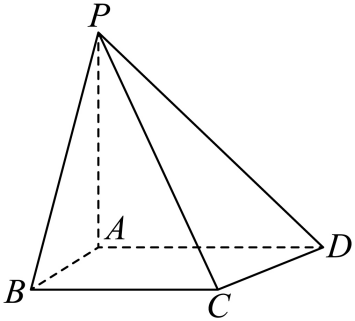
\includegraphics[width=0.9\textwidth]{image2.png}
\end{minipage}


\end{question}

\solutionSpace{5cm}
% --- 【答案】---
\begin{answer}{(1) 略；(2) (i) 略；(ii) $\dfrac{\sqrt2}{3}$。}
(1) 由 $PA\perp$ 面 $ABCD$ 推出 $AB\perp PA$，结合 $AB\perp AD$ 证 $AB\perp$ 面 $PAD$，由面面垂直判定定理得证。(2) (i) 取 $PB,PC$ 中点 $M,N$，证球心 $O$ 在平面 $ABCD$ 上；(ii) 建立坐标系 $A(0,0,0),C(\sqrt2,2,0),P(0,0,\sqrt2),O(0,1,0)$，$\cos\langle\vec{AC},\vec{PO}\rangle=\dfrac{2}{\sqrt6\cdot\sqrt3}=\dfrac{\sqrt2}{3}$。
\end{answer}

% ----------------------------------------
\begin{question}
设椭圆$C:\dfrac{x^2}{a^2}+\dfrac{y^2}{b^2}=1(a>b>0)$的离心率为$\dfrac{2\sqrt{2}}{3}$，下顶点为$A$，右顶点为$B$，$|AB|=\sqrt{10}$．

(1)求椭圆的标准方程；

(2)已知动点P不在y轴上，点R在射线AP上，且满足$\left| AR \right|\cdot \left| AP \right|=3$．

（i）设$P(m,n)$，求点$R$的坐标（用$m,n$表示）；

（ⅱ）设O为坐标原点，$M$是椭圆上的动点，直线OR的斜率为直线$OP$的斜率的3倍，求$|PM|$的最大值．

\end{question}
\solutionSpace{5cm}
% --- 【答案】---
\begin{answer}{(1) $\dfrac{x^2}{9}+y^2=1$；(2) (i) $R\left(\dfrac{3m}{m^2+(n+1)^2},\dfrac{3(n+1)}{m^2+(n+1)^2}-1\right)$；(ii) $3\sqrt3+3\sqrt2$。}
(1) 由 $e=\dfrac{2\sqrt2}{3}$，$|AB|^2=a^2+b^2=10$，解得 $a=3,b=1$。(2) (i) 由 $|AR|\cdot|AP|=3$，令 $\vec{AR}=t\vec{AP}$ 得 $R$ 坐标。(ii) 由 $k_{OR}=3k_{OP}$ 得 $P$ 在以 $(0,-4)$ 为圆心、半径 $3\sqrt2$ 的圆上，结合椭圆参数方程求得 $|PM|_{\max}=3\sqrt3+3\sqrt2$。
\end{answer}

% ----------------------------------------
\begin{question}
（1）设函数$f(x)=5\cos x-\cos 5x$,求$f(x)$在$\left[ 0,\dfrac{\pi}{4} \right]$的最大值；

（2）给定$\theta \in (0,\pi)$，设a为实数，证明：存在$y\in [a-\theta ,a+\theta ]$，使得$\cos y\le \cos \theta $；

（3）若存在$\varphi $使得对任意x，都有$5\cos x-\cos (5x+\varphi )\le b$，求b的最小值．

\end{question}
% --- 【答案】---
\begin{answer}{(1) $3\sqrt3$；(2) 略；(3) $3\sqrt3$。}
(1) $f'(x)=5(\sin5x-\sin x)=10\cos3x\sin2x$，令 $f'(x)=0$ 得 $x=\dfrac{\pi}{6}$，$f(x)_{\max}=3\sqrt3$。(2) 令 $g(y)=\cos y-\cos\theta$，则 $g(a-\theta)g(a+\theta)\le0$，故存在 $y$ 使 $\cos y\le\cos\theta$。(3) $h(x)=5\cos x-\cos(5x+\varphi)$，分析知 $h(x)_{\max}=3\sqrt3$，故 $b_{\min}=3\sqrt3$。
\end{answer}

\ifshowans\else
\newpage
\begin{center}
{\Large \textbf{参考答案}}
\end{center}
\printAnswerCheck
\fi

\end{document}
